% Fault tolerant control of a redundant cable driven parallel robot
% Elsevier CAS double column template (cas-dc), as asked by the author guide of the
% Chinese Journal of Mechanical Engineering. Compile with pdflatex and BibTeX.
\documentclass[a4paper,fleqn]{cas-dc}

\usepackage{amsmath,amssymb}
\usepackage{mathptmx}
\usepackage[scaled=0.92]{helvet}
\usepackage{courier}
\usepackage{bm}
\usepackage{booktabs,array}
\usepackage{graphicx}
\usepackage{adjustbox}
\usepackage{placeins}
\usepackage{algorithm}
\usepackage[noend]{algpseudocode}
\usepackage[numbers,sort&compress]{natbib}

\graphicspath{{figures/}{../figures/}}
\newcommand{\tablefile}[1]{\IfFileExists{tables/#1.tex}{\input{tables/#1}}{\input{../tables/#1}}}
\newcommand{\vc}[1]{\bm{#1}}
\newcommand{\mt}[1]{\mathbf{#1}}
\newcommand{\sk}[1]{[#1]_{\times}}
\newcommand{\eye}{\mt{I}}
\renewcommand{\algorithmicrequire}{\textbf{Every 1 ms:}}

% cas-common.sty joins the author names on the highlights page without a space
\ExplSyntaxOn
\RenewDocumentEnvironment { PrelimsAbstract } { O{} }
  { \parindent=0pt
    { \fontsize{14pt}{16pt}\selectfont #1 } \par
    \vskip12pt
    { \fontsize{12pt}{14pt}\bfseries\selectfont\casprelimstitle } \par
    \vskip6pt
    \int_compare:nNnTF { \value{blind} } > { 0 }
      { \vspace*{\the\baselineskip} }
      { \seq_use:Nn \g_stm_prelimsau_seq { ,~ } }
    \vskip12pt
    \par }
  { }
\ExplSyntaxOff

\begin{document}
\let\WriteBookmarks\relax
\def\floatpagepagefraction{1}
\def\textpagefraction{.001}

\shorttitle{Fault tolerant control of a redundant cable driven parallel robot}
\shortauthors{M.\,J. Tachia, A.\,V. Maloletov}

\title[mode=title]{Fault tolerant control of a redundant cable driven parallel robot with model based fault isolation and precomputed recovery plans}

\author[1]{Mfeuter Joseph Tachia}[orcid=0000-0002-9274-3658]
\cormark[1]
\ead{m.tachia@innopolis.university}
\author[1,2]{Alexander V. Maloletov}[orcid=0000-0002-7312-2944]
\affiliation[1]{organization={Institute of Robotics and Computer Vision, Innopolis University},
  addressline={Universitetskaya St. 1}, city={Innopolis}, postcode={420500}, country={Russia}}
\affiliation[2]{organization={Volgograd State Technical University},
  addressline={Lenin Avenue 28}, city={Volgograd}, country={Russia}}
\cortext[1]{Corresponding author}

\begin{abstract}
A cable driven parallel robot that loses a cable has a fraction of a second to move its platform to a pose that the remaining cables can still hold. We present a fault tolerant controller for the eight cable robot IPAnema~2 that identifies the fault from the motor encoders and currents of the winches alone and answers a cable break with a recovery motion computed in advance. Extended state observers estimate the cable tensions at each winch, and an interacting multiple model estimator over seventeen modes separates cable breaks from actuator faults at the platform. A model predictive controller tracks the task within the tension bounds and, once a break is declared, follows a stored optimal recovery path that brings the platform to rest at a pose the seven remaining cables can hold. The controller was compared with eight alternatives in a paired simulation study of 624 fault cases and 200 fault free runs on randomised robots with elastic cables, winch dynamics and sensor noise. It identified 623 of the 624 faults correctly, declared every cable break within 19~ms and lost the platform after 11 of 208 cable breaks, against 122 without fault tolerance and 65 with a classical threshold based pipeline. A recurrent neural classifier trained on the same signals identified faults later and less reliably and raised frequent false alarms, and when its probabilities also shaped the constraints of the controller, the platform was lost after 44 of 64 breaks. Weighting the fault scenarios of the controller by their probabilities before a declaration, the idea this study set out to test, gave no measurable benefit, because the model based diagnosis declares a cable break within one control period. The controller does not yet run in real time, which is the main step before tests on hardware.
\end{abstract}

\begin{highlights}
\item A 17 mode IMM isolates every cable break within 19 ms from winch signals alone
\item Recovery plans computed offline keep the platform after 197 of 208 cable breaks
\item A learned fault classifier should not shape the constraints of the controller
\item Probability weighted MPC gave no benefit, as breaks are declared within one period
\end{highlights}

\begin{keywords}
Cable driven parallel robot \sep Fault tolerant control \sep Fault isolation \sep Interacting multiple model \sep Model predictive control \sep Cable failure \sep Recovery planning
\end{keywords}

\maketitle

% =====================================================================
\section{Introduction}\label{sec:intro}

A cable driven parallel robot can lose a cable in the middle of a task, and when it does, the platform starts to fall before any controller has noticed. These robots move a platform with cables wound on winches fixed to a frame, which gives them a workspace of several metres, a light moving mass and a payload that rigid parallel robots of the same size cannot reach \citep{pott2018book,qian2018review,tachia2026review}. These properties are the reason they are considered for building facades, large scale additive manufacturing and other construction tasks \citep{izard2017printing}, and they are also the reason a failure is dangerous: a platform of several kilograms hangs metres above the floor, held by thin cables and by drives that run for hours. A cable can break, and a winch can lose part of its torque or develop a parasitic one. In a fully constrained robot with eight cables and six degrees of freedom the loss of one cable does not make the platform uncontrollable at once, but it removes most of the poses at which the remaining cables can hold it. For the robot of this study, IPAnema~2 \citep{pott2013ipanema}, no level pose near the task can be held after an upper cable breaks (Section~\ref{sec:workspace}), and without a fault tolerant reaction the platform was lost after every one of 104 simulated breaks of an upper cable. Recovering from a break is therefore a race. The controller has to find out which cable has gone, decide where the platform can still be held and start moving it there within a few tenths of a second, while the platform is already falling.

Most work on cable failures asks what the robot can still do once the failure is known. \citet{roberts1998fault} studied the fault tolerance of cable suspended robots through their statics, and \citet{notash2012failure} gave criteria under which the wrench capability of a wire actuated manipulator is fully or partly recovered after a failure. For the motion after a break, \citet{berti2016recovery} moved the point mass of a redundant suspended robot from the unstable pose left by the failure to a new static equilibrium, \citet{passarini2019camera} drove a cable suspended camera toward a safe landing pose along an oscillatory trajectory that keeps the remaining tensions positive and bounded, and \citet{boschetti2019rehab} stopped a rehabilitation robot with a wrench opposed to its motion. \citet{boumann2019emergency} developed emergency strategies that minimise the kinetic energy of the platform or steer it with potential fields, and validated them later on a prototype \citep{boumann2023validation}, while \citet{dipaola2024smapid} guided the load inside the remaining wrench feasible workspace with a sliding mode adaptive PID control. These strategies take the failure as known at its onset, and most of them were shown on planar or point mass models or on suspended robots. For a spatial, fully constrained robot two questions are left open: how the delay and the reliability of the diagnosis shape the outcome, and how a recovery motion of the full six degree of freedom pose, which has to be dynamically feasible with seven cables, can be ready within the few tenths of a second the platform leaves.

Banks of mode matched filters combined by the interacting multiple model (IMM) estimator \citep{blom1988imm} have long been used to detect and isolate actuator and sensor failures \citep{zhang1998imm,zhang2008review}. In cable driven robots the diagnosis has received less attention than the recovery. \citet{raman2023cable} isolated cable failures of a planar reconfigurable robot with an IMM bank of extended Kalman filters, assuming that the platform pose is measured. \citet{majdi2023smc} detected partial actuator losses of a planar robot with an extended state observer, and \citet{fazeli2023active} estimated actuator faults with an adaptive observer inside a finite time sliding mode controller and verified the scheme on a planar robot. \citet{bettega2025load} estimated the load torque of each motor from its current and encoder and detected cable failures with machine learning classifiers. Learned detectors need no model of the faulty robot, but they know only the behaviour represented in their training data \citep{khalastchi2018survey}, and in a fault tolerant controller that behaviour changes as soon as the controller acts on the detector. None of these works isolates both cable breaks and actuator faults of a spatial robot from the winch signals alone, and we have not found a comparison of a learned and a model based diagnosis inside the same closed loop.

Model predictive control (MPC) suits cable robots because the tension bounds become constraints of the optimisation instead of being left to a separate tension distribution step \citep{gouttefarde2015tda}. \citet{santos2022nmpc} built the tension distribution into a nonlinear MPC with conditions for stability, \citet{song2022wmpc} used an offline workspace analysis to give the online problem convex constraints and recursive feasibility, and \citet{gao2025dobmpc} combined MPC with a disturbance observer. When the model itself is uncertain, multistage MPC optimises one input sequence against several candidate models at once \citep{lucia2013multistage}. A diagnosis that returns mode probabilities suggests combining the two: before a fault is confirmed, the controller could already weigh what each plausible fault would do and move the platform toward poses that would survive it. This was the hypothesis our study began with, and here it is tested as an ablation.

This paper presents and evaluates a fault tolerant controller for IPAnema~2 on a simulator that integrates elastic and unilateral cables, the winch dynamics, sensor quantisation and noise and randomised parameters, while the controller works with a rigid cable model. An extended state observer at each winch estimates the cable tension from the encoder and the motor current, and an IMM over seventeen modes, the healthy robot, eight cable breaks and eight actuator faults, separates breaks from actuator faults at the platform. An MPC tracks the task within the tension bounds, and after a break is declared it follows a recovery plan, the solution of an optimal control problem on the seven cable model computed in advance along the known task. All methods ran on the same randomised runs, with the endpoints, the statistics and the settings of every method fixed before any evaluation run. The contributions are three.
\begin{enumerate}
\item A two level diagnosis that isolates cable breaks, losses of effectiveness and torque biases of a spatial robot from the encoders and motor currents of the winches, without load cells or a pose sensor. It identified 623 of 624 faults correctly and declared every break within 19~ms.
\item A library of recovery plans computed offline along the task and selected at the declaration, which removes the latency of solving the plan online. With it the platform was lost after 11 of 208 breaks, against 20 with the same planner solved online and 122 without fault tolerance.
\item Evidence from a paired comparison that a learned diagnosis, trained on the same signals, should not shape the constraints of the controller: used that way it raised false alarms in 154 of 252 runs and lost 44 of 64 breaks.
\end{enumerate}
The probability aware weighting of the MPC had no measurable effect with the IMM, and we report it as an ablation together with its reason.

The argument runs from the robot to the evaluation. Section~\ref{sec:model} derives the model of IPAnema~2 and shows what a cable break leaves of its workspace, which fixes what the controller must do. Sections~\ref{sec:diagnosis} and \ref{sec:control} build the diagnosis and the controller on that model, Section~\ref{sec:evaluation} describes how they were evaluated against eight alternatives, Section~\ref{sec:results} gives the results, and Section~\ref{sec:discussion} discusses what they show and where the study stops.

% =====================================================================
\section{Robot, model and faults}\label{sec:model}

\subsection{The robot}\label{sec:robot}

IPAnema~2 is a member of a family of industrial cable robots, built in a frame of $8\times6\times5$~m \citep{pott2013ipanema}. We use its geometry, mass, inertia and upper tension bound as distributed with the IPAnema~2 model of the open source toolkit CASPR \citep{lau2016caspr}, whose geometry coincides with the published one, and its cables, winches and drives as published (Table~\ref{tab:parameters}). Anchor $i$ is at $\vc a_i=(4\sigma_{x,i},\,3\sigma_{y,i},\,z_{a})$~m, with $z_a=5$~m for the upper cables 1 to 4 and $z_a=1$~m for the lower cables 5 to 8, and the cable is attached to the platform at $\vc b_i=(0.65\sigma_{x,i},\,0.125\sigma_{y,i},\,0.25)$~m for the upper and $(0.75\sigma_{x,i},\,0.10\sigma_{y,i},\,0.75)$~m for the lower cables, where the signs $(\sigma_{x,i},\sigma_{y,i})$ are $(-,+)$, $(+,+)$, $(+,-)$ and $(-,-)$ for cables 1 to 4 and, in the same order, for cables 5 to 8. The platform of 10~kg has its centre of mass 0.5~m above its reference point $P$, the point that follows the task, and the home pose places $P$ at $(0,0,3)$~m with zero orientation (Fig.~\ref{fig:robot}). With eight cables pulling upward and downward at the same time the platform resists a wrench in any direction while every cable stays in tension. The redundancy is two, which leaves a two dimensional family of tension distributions for every wrench, and after the loss of one cable it drops to one.

\tablefile{tab_parameters}

\begin{figure}[t]
\centering
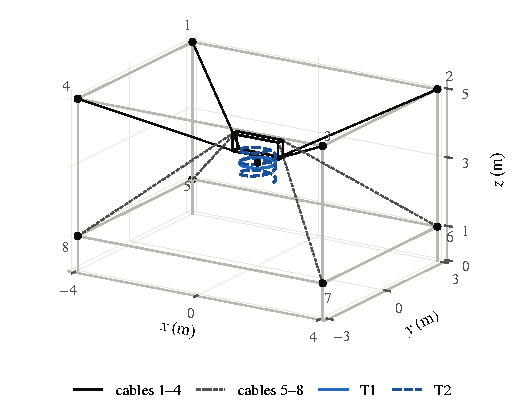
\includegraphics[width=\columnwidth]{fig01_robot_task.pdf}
\caption{IPAnema~2 at its home pose, with the eight cables (upper anchors at $z=5$~m, lower anchors at $z=1$~m), the reference point P of the platform and the two reference paths: the circle T1 and the helix T2, both 16~s long.}\label{fig:robot}
\end{figure}

\subsection{Kinematics}\label{sec:kinematics}

The world frame has its $z$ axis pointing upward. The pose of the platform is described by the generalised coordinates
\begin{equation}\label{eq:q}
\vc q=\begin{bmatrix}\vc p\\ \vc\varphi\end{bmatrix}\in\mathbb R^{6},\qquad \mt R(\vc\varphi)=\mt R_z(\psi)\,\mt R_y(\vartheta)\,\mt R_x(\phi),
\end{equation}
where $\vc p$ is the position of $P$ and $\vc\varphi=[\phi,\vartheta,\psi]^\top$ are ZYX Euler angles. Each cable is taken to leave the frame at its fixed anchor point, and the small motion of the exit point on the guiding pulley is neglected. The angular velocity follows from the Euler rates as $\vc\omega=\mt E(\vc\varphi)\dot{\vc\varphi}$, with $\mt E$ singular only at $\vartheta=\pm\pi/2$, far outside the tilt this robot can hold, and we collect the velocities in the twist $\vc\nu=[\dot{\vc p}^\top,\vc\omega^\top]^\top=\mt H(\vc q)\dot{\vc q}$ with $\mt H=\operatorname{blkdiag}(\eye_3,\mt E)$. Cable $i$ runs from the attachment point to the anchor, so its vector, length and direction are
\begin{equation}\label{eq:cable}
\vc l_i=\vc a_i-\vc p-\mt R\vc b_i,\qquad l_i=\lVert\vc l_i\rVert,\qquad \vc u_i=\vc l_i/l_i,
\end{equation}
and a tension $t_i\ge0$ acts on the platform as the force $t_i\vc u_i$. Differentiating \eqref{eq:cable} gives, for all cables together,
\begin{equation}\label{eq:ldot}
\dot{\vc l}=-\mt W^\top\vc\nu,\qquad
\mt W=\begin{bmatrix}\vc u_1&\cdots&\vc u_n\\ (\mt R\vc b_1)\times\vc u_1&\cdots&(\mt R\vc b_n)\times\vc u_n\end{bmatrix},
\end{equation}
where $\mt W\in\mathbb R^{6\times n}$ is the wrench matrix: the cables apply to the platform the force and the moment about $P$ given by $\mt W\vc t$. The same matrix, transposed and with a minus sign, maps the twist to the rates of the cable lengths, and the sign in \eqref{eq:ldot} is the one that keeps the cables pulling.

\subsection{Dynamics from the Lagrange equations}\label{sec:lagrange}

We treat the platform as a rigid body and the cables, in this subsection, as sources of generalised forces. With $\vc c_w=\mt R\vc c$ the position of the centre of mass relative to $P$, the kinetic and potential energies are
\begin{align}
T&=\tfrac12 m\lVert\dot{\vc p}+\vc\omega\times\vc c_w\rVert^2+\tfrac12\vc\omega^\top\mt I_c\vc\omega=\tfrac12\dot{\vc q}^\top\mt M(\vc q)\dot{\vc q},\label{eq:T}\\
V&=m g\,\vc e_3^\top(\vc p+\mt R\vc c),\label{eq:V}
\end{align}
where $\mt I_c=\mt R\mt I_G\mt R^\top$ is the inertia about the centre of mass in world coordinates, and expanding the square gives
\begin{equation}\label{eq:M}
\mt M=\mt H^\top\mt M_\nu\mt H,\qquad
\mt M_\nu=\begin{bmatrix}m\eye_3&-m\sk{\vc c_w}\\ m\sk{\vc c_w}&\mt I_c-m\sk{\vc c_w}^2\end{bmatrix},
\end{equation}
with $\sk{\cdot}$ the cross product matrix. The off diagonal blocks couple translation and rotation because $P$ is not the centre of mass, and with an offset of 0.5~m this coupling is far from small. The elastic energy of the cables is deliberately left out of $V$: the cable forces enter once, through their virtual work, so that they cannot be counted both as a potential and as an applied force. A virtual displacement moves attachment point $i$ by $\delta\vc p+\delta\vc\Theta\times\mt R\vc b_i$ with $\delta\vc\Theta=\mt E\,\delta\vc\varphi$, and the virtual work of the tensions,
\begin{equation}\label{eq:Q}
\delta W=\sum_{i=1}^n t_i\vc u_i^\top(\delta\vc p+\delta\vc\Theta\times\mt R\vc b_i)=(\mt H^\top\mt W\vc t)^\top\delta\vc q,
\end{equation}
gives the generalised force $\vc Q=\mt H^\top\mt W\vc t=-(\partial\vc l/\partial\vc q)^\top\vc t$, which says that a tension does negative work when its cable gets longer. The Lagrange equations of $L=T-V$ then read
\begin{equation}\label{eq:EL}
\mt M(\vc q)\ddot{\vc q}+\mt C(\vc q,\dot{\vc q})\dot{\vc q}+\vc G(\vc q)=\mt H^\top\mt W\vc t,
\end{equation}
where $\vc G=\partial V/\partial\vc q=-\mt H^\top\vc w_g$ with the gravity wrench $\vc w_g=[m\vc g^\top,\ (\vc c_w\times m\vc g)^\top]^\top$, and $\mt C$ is built from the Christoffel symbols of the first kind,
\begin{equation}\label{eq:C}
C_{kj}=\sum_{i=1}^{6}\frac12\Big(\frac{\partial M_{kj}}{\partial q_i}+\frac{\partial M_{ki}}{\partial q_j}-\frac{\partial M_{ij}}{\partial q_k}\Big)\dot q_i,
\end{equation}
the choice that makes $\dot{\mt M}-2\mt C$ skew symmetric. Substituting $\dot{\vc q}=\mt H^{-1}\vc\nu$ and multiplying by $\mt H^{-\top}$ gives the Newton--Euler form about $P$,
\begin{equation}\label{eq:NE}
\begin{gathered}
\mt M_\nu\dot{\vc\nu}+\vc b(\vc q,\vc\nu)=\mt W\vc t+\vc w_g,\\
\vc b=\begin{bmatrix}m\,\vc\omega\times(\vc\omega\times\vc c_w)\\ \vc\omega\times\mt I_c\vc\omega+m\,\vc c_w\times\big(\vc\omega\times(\vc\omega\times\vc c_w)\big)\end{bmatrix},
\end{gathered}
\end{equation}
which has no Euler angle singularity in its mass matrix and is cheaper to evaluate. The simulator integrates \eqref{eq:NE} with the orientation carried as a unit quaternion, so that it stays regular through the large rotations of an uncontrolled platform, and the estimators and the controller use the same equation with the tensions as inputs. We checked the derivation against a symbolic Lagrangian and the two forms against each other numerically (Appendix~\ref{app:verification}).

\subsection{Cables and winches}\label{sec:cables}

Each cable is wound on a drum that a motor turns through a gearbox. With the motor angle $\theta_i$ taken positive when cable is reeled in, the unstretched free length is $l_{u,i}=l^0_{u,i}-r_d\theta_i$, where $r_d=r_D/i_g=50~\text{mm}/12=4.167$~mm/rad is the cable paid out per radian of the motor shaft. With the stretch $\Delta_i=l_i-l_{u,i}$ and the axial stiffness $k_i=EA/l_{u,i}$, the tension follows a Kelvin--Voigt law cut off at zero,
\begin{equation}\label{eq:tension}
t_i=\begin{cases}\max\!\big(0,\ k_i\Delta_i+\beta k_i\,s(\Delta_i)\,\dot\Delta_i\big),&\Delta_i>0,\\ 0,&\Delta_i\le0,\end{cases}
\end{equation}
where $\beta$ is a retardation time. The cut off is what makes a cable a cable: it pulls but cannot push, and once slack it carries no load until it is stretched again. The factor $s(\Delta)=3r^2-2r^3$, $r=\min(\Delta/\Delta_s,1)$ with $\Delta_s=0.1$~mm, lets the damping grow from zero with the stretch, as \citet{hunt1975coefficient} proposed for impacts, so that a cable which tightens again does not jump at once to the force $\beta k\dot\Delta$. No stiffness has been published for the 1.5~mm Dyneema cables of IPAnema~2. We scaled the values identified on the 6~mm cable of IPAnema~3 \citep{tempel2015iftomm} by the ratio of the cross sections, which gives $EA=35.2$~kN, kept the retardation time of 0.02~s, and randomised $EA$ by $\pm20\%$ in every run because the value is scaled and not measured. At the home pose the six elastic modes of the platform with locked winches then lie between 5.5 and 18.7~Hz. The cables are taken as straight: over the feasible workspace the equivalent modulus of a sagging cable \citep{ernst1965} never falls below 95.4\% of $EA$. This is a property of the light cable of this robot. With heavier cables the sag changes the cable forces noticeably, and models that combine the Kelvin--Voigt elasticity with a catenary have been used to compensate it with a learned controller \citep{tachia2025sac}.

Every winch carries a synchronous servo motor of the Bosch Rexroth IndraDyn~S series with a multi turn absolute encoder, a planetary gearbox with $i_g=12$ and a drum of 100~mm diameter that stores 6~m of cable \citep{pott2013ipanema}. The motor size of IPAnema~2 is not published, and we took the MSK030C, the smallest motor of the series that reaches the speed and the holding torque the robot needs \citep{rexroth_msk2018}. Referred to the motor shaft, the winch obeys
\begin{equation}\label{eq:winch}
I_m\ddot\theta_i=\tau_i^{\mathrm{act}}-r_d t_i,
\end{equation}
where $\tau_i^{\mathrm{act}}$ is the torque the motor delivers and $I_m$ the rotor inertia; friction is left out, as in the winch analysis of \citet{ida2022actuators}, because no data on it are published. The winch is not small next to the platform: seen from the cable, the rotor of 0.3~kg\,cm$^2$ acts like a mass of $I_m/r_d^2=1.7$~kg, against a platform of 10~kg. Equation \eqref{eq:winch} is the Lagrange equation of the coordinate $\theta_i$, with the kinetic energy $\tfrac12I_m\dot\theta_i^2$ and the virtual work $(\tau_i^{\mathrm{act}}-r_dt_i)\,\delta\theta_i$ of the motor and the cable on the drum, so that \eqref{eq:EL} and \eqref{eq:winch} together are the Lagrange equations of the robot in the coordinates $(\vc q,\vc\theta)$. The drum limits the change of the free length to 6~m, a window that we centred on the lengths each cable takes over the static workspace. Equations \eqref{eq:NE}, \eqref{eq:tension} and \eqref{eq:winch} form the model of the simulator.

\subsection{Faults and sensors}\label{sec:faults}

Three faults are described by one parameterisation,
\begin{equation}\label{eq:fault}
\tau_i^{\mathrm{act}}=(1-\rho_i)\,\tau_i+f_i,\qquad t_i\equiv0\ \text{for } t\ge t_f\ \text{if cable } i \text{ breaks},
\end{equation}
where $\tau_i$ is the torque the drive applies. A break removes the cable for good, a loss of effectiveness $\rho_i\in(0,1)$ models a drive that delivers only part of its torque, for instance through a damaged gear stage, and a bias $f_i$ models a constant parasitic torque such as a dragging brake.

The robot carries no load cells and no sensor of the platform pose. Each winch reports its motor angle, from the encoder, and its motor current, which the torque constant turns into the torque $\tau_i$; on the IPAnema robots the same current is used to estimate the cable tension \citep{pott2013ipanema}. This choice is deliberate. With a load cell on every cable a break would show as a zero reading and the diagnosis would be trivial, whereas without load cells the tension has to be inferred from the motor side, and a loss of effectiveness becomes invisible to the drive, whose current is correct while its torque is not. The encoder resolves $2^{20}$ counts per revolution with an error of $\pm120''$ \citep{rexroth_msk2018}, and the torque measurement carries white noise of 0.004~N\,m, a value we chose because none is published and which the evaluation doubles in half of the runs. The controller runs at 1~kHz and receives every reading one sample late.

\subsection{What a cable break leaves}\label{sec:workspace}

For a set $\mathcal S$ of intact cables, a pose is statically feasible when every free length lies in its drum window and the cables of $\mathcal S$ balance gravity with tensions inside $[t_{\min},t_{\max}]$. How far inside that set a pose lies is measured by the margin
\begin{equation}\label{eq:margin}
\begin{aligned}
s^\star(\vc q,\mathcal S)=\max_{s,\,\vc t_{\mathcal S}}\ s\quad\text{s.t.}\quad&\mt W_{\mathcal S}\vc t_{\mathcal S}+\vc w_g=\vc 0,\\
&t_{\min}+s\le t_i\le t_{\max}-s,
\end{aligned}
\end{equation}
a linear programme whose solution is also the tension distribution farthest from both bounds. On a grid of 0.25~m over the interior of the frame, the eight cables hold the level platform at 3,357 positions within the drum windows. After the loss of one upper cable 11.8\% of these positions remain, and after the loss of a lower cable 42.2\%. Fig.~\ref{fig:workspace} shows two slices through the paths. In the horizontal plane $z=3$~m, where the circular task lies, 8,059 of 14,241 points of a 0.05~m grid are feasible with all cables, 14 after the loss of the upper cable~1 and 4,073 after the loss of the lower cable~5.

\begin{figure*}[t]
\centering
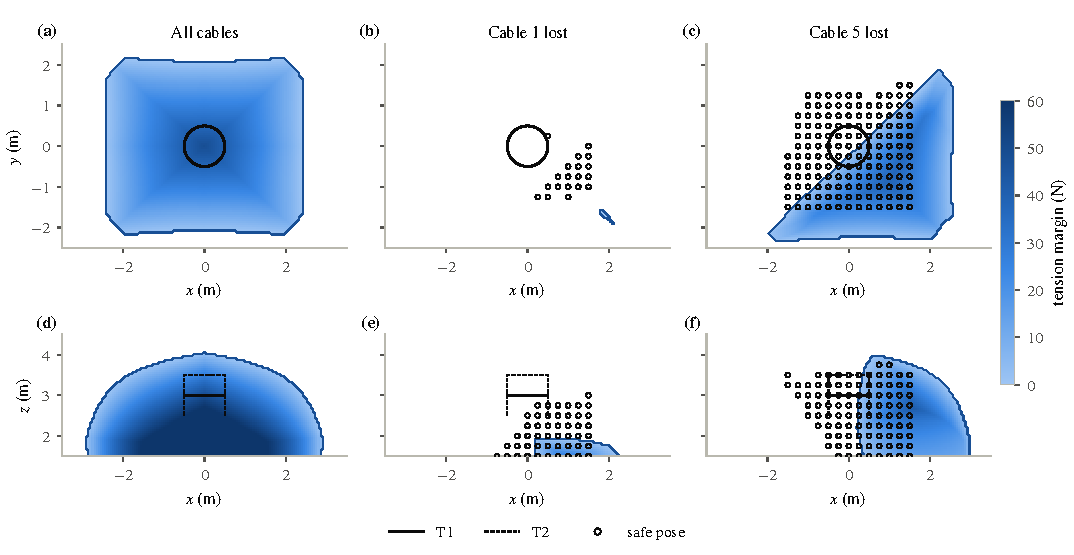
\includegraphics[width=\textwidth]{fig02_postfault_workspace.pdf}
\caption{A cable break leaves the level platform almost no pose near the task when the lost cable is an upper one. Shading: tension margin \eqref{eq:margin} of the level platform at the poses where all remaining cables stay within $[t_{\min},t_{\max}]=[10,200]$~N and within their drum windows, in the horizontal plane $z=3$~m (a--c) and the vertical plane $y=0$ (d--f), with all cables (a, d), after the loss of the upper cable~1 (b, e) and after the loss of the lower cable~5 (c, f). Circles: poses in the same plane that the remaining cables hold with a margin of at least 10~N once the platform may tilt by up to $20^\circ$; these are the targets of the recovery plans. Lines: the path T1 and the extent of the helix T2.}\label{fig:workspace}
\end{figure*}

The robot keeps more of its workspace when the platform may give up its orientation. Allowing a tilt of up to $20^\circ$ about each axis, 52.3\% of the positions can be held after an upper cable breaks and 73.8\% after a lower one, with a median tilt of $10^\circ$. Tilting is therefore the main resource the robot has left after a break. Redistributing the tensions and carrying on is not an option, since for most of the workspace there is no distribution to carry on with; the platform has to be moved and tilted into the feasible set of the cables that remain, and the motion has to start before that set is out of reach.

The two reference paths of the evaluation lie in the centre of the workspace (Fig.~\ref{fig:robot}). T1 is a horizontal circle of 0.5~m radius at $z=3$~m with a period of 4~s, followed for three turns in 16~s, and the helix T2 follows the same circle while climbing from $z=2.5$ to 3.5~m. The peak speed of 0.79~m/s is a third of the speed limit of the robot. On neither path can the level platform be held at any point after an upper cable breaks, while after a lower cable breaks it can on 29 to 52\% of the path, depending on the cable. An upper cable break therefore always forces the platform to leave its orientation, and a lower cable break sometimes leaves the task possible at a lower speed.

% =====================================================================
\section{Fault diagnosis}\label{sec:diagnosis}

The diagnosis has to tell eight cable breaks and eight actuator faults apart from the encoders and motor currents, and it has to do it in a few tens of milliseconds. It works on two levels because the two kinds of fault leave their signatures in different places.

\subsection{Tension estimation at each winch}\label{sec:eso}

Writing \eqref{eq:winch} with \eqref{eq:fault} as $\ddot\theta_i=b_0\tau_i+d_i$ with $b_0=1/I_m$ gathers everything that is not the commanded torque into one unknown, $d_i=-(r_dt_i+\rho_i\tau_i-f_i)/I_m$. An extended state observer \citep{han2009pid} treats $d_i$ as a third state and estimates it from the encoder,
\begin{equation}\label{eq:eso}
\begin{aligned}
\dot z_{1,i}&=z_{2,i}+3\omega_o(\tilde\theta_i-z_{1,i}),\\
\dot z_{2,i}&=z_{3,i}+b_0\tau_i+3\omega_o^2(\tilde\theta_i-z_{1,i}),\\
\dot z_{3,i}&=\omega_o^3(\tilde\theta_i-z_{1,i}),
\end{aligned}
\end{equation}
with all observer poles at $-\omega_o$ \citep{gao2003scaling}, and the tension estimate is $\hat t_i=-I_m z_{3,i}/r_d$. For a bounded rate of $d_i$ the error of such an observer is ultimately bounded, with a bound that shrinks as $\omega_o$ grows \citep{guo2011eso}, but $\omega_o$ cannot grow freely, because the third channel amplifies the encoder quantisation by $\omega_o^3$. With $\omega_o=2\pi\cdot50$~rad/s the estimate followed the cable tension of the plant with an RMS error of 0.30~N at the nominal current noise and 0.57~N at twice that noise, at the price of a lag of $3/\omega_o=9.5$~ms. Comparing $d_i$ with $z_{3,i}$, the estimate converges to
\begin{equation}\label{eq:bias}
\hat t_i\ \to\ t_i+\frac{\rho_i\tau_i-f_i}{r_d}.
\end{equation}
This relation is the reason the diagnosis needs two levels. A cable break is seen at the winch, because $t_i$, and with it $\hat t_i$, drops to zero while the commanded tension does not. An actuator fault is not seen there, because it adds to $\hat t_i$ exactly the torque the motor failed to deliver: a tension loop closed on $\hat t_i$ holds the estimate at its reference while the true tension is lower by the deficit $\delta_i=(\rho_i\tau_i-f_i)/r_d$. The deficit acts on the platform, and the platform is where it has to be found. Each winch tracks the tension $t_{d,i}$ requested by the controller with
\begin{equation}\label{eq:loop}
\tau_i=r_dt_{d,i}+I_m\ddot\theta_i^{\,\mathrm{ff}}+r_d\Big(k_Pe_i+k_I\!\int e_i\,dt\Big),\qquad e_i=t_{d,i}-\hat t_i,
\end{equation}
where $\ddot\theta_i^{\,\mathrm{ff}}$ is the drum acceleration implied by the motion the controller predicts.

\subsection{Interacting multiple model estimator}\label{sec:imm}

The platform level diagnosis runs an IMM estimator \citep{blom1988imm} over the $N=2n+1=17$ modes $\mathcal M_0$ (healthy), $\mathcal B_i$ (break of cable $i$) and $\mathcal A_i$ (actuator fault of winch $i$). Each mode states which tensions the platform receives for a commanded vector $\vc t_d$,
\begin{equation}\label{eq:modes}
\vc t^{(0)}=\vc t_d,\qquad \vc t^{(\mathcal B_i)}=(\eye-\vc e_i\vc e_i^\top)\vc t_d,\qquad \vc t^{(\mathcal A_i)}=\vc t_d-\vc e_i\delta_i,
\end{equation}
where $\delta_i$ is the unknown deficit of \eqref{eq:bias}. The mode $\mathcal A_i$ merges the loss of effectiveness and the bias, because both produce the same signature at the platform. Every filter carries the state $\vc x=[\vc q^\top,\vc\nu^\top,\delta,\vc w_b^\top,\vc\eta^\top,\gamma]^\top\in\mathbb R^{28}$. The deficit $\delta$ is a random walk used only by the modes $\mathcal A_i$. The other three groups describe what the nominal model gets wrong and are shared by all modes: $\vc w_b$ is a slowly varying wrench that absorbs the errors in mass, centre of mass and inertia, $\vc\eta$ holds offsets of the length readings that absorb the errors of the anchors and of the homing, and $\gamma$ is the ratio of the true to the nominal axial stiffness. They are needed because the deficit of a mode $\mathcal A_i$ is a free parameter: without them, on a randomised plant, the filters of the actuator modes absorbed the model mismatch and won in fault free runs. A fault, in contrast, is an abrupt change that the slow bias states cannot follow on the time scale of the diagnosis, so it remains for the fault modes to explain.

Each filter propagates the mean of \eqref{eq:NE}, with its own $\vc t^{(j)}$ and the wrench $\vc w_b$ added, over the period $\Delta_I=5$~ms by a fourth order Runge--Kutta step, and the covariance with the Jacobian obtained by algorithmic differentiation. The measurement is $\vc y=[\tilde{\vc l}_u^\top,\hat{\vc t}^\top]^\top$, the unstretched lengths read from the encoders and the tension estimates of the winches, and under mode $j$ its expected value is
\begin{equation}\label{eq:h}
\tilde l_{u,i}=\frac{\gamma EA\,l_i(\vc q)}{\gamma EA+t_i^{(j)}}+\eta_i,\qquad
\hat t_i=\begin{cases}0,&j=\mathcal B_i,\\ t_{d,i},&\text{otherwise},\end{cases}
\end{equation}
where the first relation is \eqref{eq:tension} solved for the free length and the second states that the tension loop holds $\hat t_i$ at its reference unless the cable has gone. The filters take the tension commands, averaged over the period, as their input rather than the tension estimates, which lag the true tensions by 9.5~ms; this also gives the IMM a model of the motion the controller itself produces. The fault modes enter only after the first 2~s, which gives the bias states time to converge at the start of the task.

Let $\pi_{lj}$ be the probability of switching from mode $l$ to mode $j$ in one period and $\mu_l$ the mode probabilities after the previous period. One cycle computes the predicted probabilities and the mixing weights,
\begin{equation}\label{eq:mix}
\bar c_j=\sum_l\pi_{lj}\mu_l,\qquad\mu_{l|j}=\pi_{lj}\mu_l/\bar c_j,
\end{equation}
mixes the states that all filters share, runs the extended Kalman prediction and update of each filter, and obtains its innovation $\vc r^{(j)}$ with covariance $\mt S^{(j)}$. The likelihood of mode $j$ is the Gaussian density of its innovation, and the probabilities follow from Bayes' rule,
\begin{equation}\label{eq:mu}
\begin{gathered}
\ln\Lambda^{(j)}=-\tfrac12\big(\vc r^{(j)\top}\mt S^{(j)-1}\vc r^{(j)}+\ln\det(2\pi\mt S^{(j)})\big),\\
\mu_j=\frac{\Lambda^{(j)}\bar c_j}{\sum_l\Lambda^{(l)}\bar c_l}.
\end{gathered}
\end{equation}
We evaluate \eqref{eq:mu} in the log domain, subtracting the largest $\ln\Lambda^{(l)}+\ln\bar c_l$ before exponentiating. This is not a detail. A cable break produces innovations of tens of newtons, the densities of all modes then underflow in double precision, and a direct evaluation returns $0/0$ or falls back on the prior, after which the probabilities only follow the Markov chain. In the log domain $\mu_j\ge0$ and $\sum_j\mu_j=1$ hold at every step, and the code asserts both. A fault is declared when one mode $j\ne0$ holds $\mu_j\ge\mu_{\mathrm{iso}}$ for $N_c$ consecutive cycles. The noise levels, the switching rates and the pair $\mu_{\mathrm{iso}}=0.9999$, $N_c=2$ are listed in Table~\ref{tab:settings}, with those chosen on calibration runs marked.

\begin{table*}[t]
\centering\small
\caption{Settings of the estimators and the controller. Design: chosen and stated, not tuned; calibrated: chosen on calibration runs by rules written before those runs.}\label{tab:settings}
\begin{tabular}{@{}>{\raggedright\arraybackslash}p{0.17\textwidth}>{\raggedright\arraybackslash}p{0.33\textwidth}>{\raggedright\arraybackslash}p{0.24\textwidth}>{\raggedright\arraybackslash}p{0.18\textwidth}@{}}
\toprule
Part & Setting & Value & Source\\
\midrule
Winch observer and loop & bandwidth $\omega_o/2\pi$; $k_P$, $k_I$ & 50~Hz; 0.5, 20~s$^{-1}$ & design\\
IMM & period; arming time & 5~ms; 2~s & design\\
 & process noise, linear and angular acceleration & 0.5~m\,s$^{-2}$, 1~rad\,s$^{-2}$ & design; calibrated\\
 & measurement noise, lengths and tensions & 0.2~mm, 1.5~N & design\\
 & deficit random walk; fault and return rates & 20~N\,s$^{-1/2}$; $10^{-3}$, $10^{-2}$~s$^{-1}$ & design\\
Declaration & $\mu_{\mathrm{iso}}$, $N_c$ & 0.9999, 2 & calibrated\\
MPC & period, horizon & 20~ms, 12 steps & design\\
 & weights: pose; velocity; tension change & $4\times10^4$; 120; 0.03 & calibrated\\
 & after a break declaration & velocity $\times0.3$, tension change $\times3$ & calibrated\\
 & scenarios: threshold $\mu_s$, at most & $10^{-3}$, 2 fault scenarios & design\\
Planner & time scaling: horizon, $\kappa_{\min}$ & 2~s, 0.25 & design\\
 & recovery \eqref{eq:recovery}: $T$, intervals; $s_p$, $s_{\min}$ & 1~s, 15; 5, 10~N & design\\
 & library: break instants; detection delay & every 50~ms; 15~ms & design\\
\bottomrule
\end{tabular}
\end{table*}

% =====================================================================
\section{Control and recovery}\label{sec:control}

Fig.~\ref{fig:architecture} shows how the parts fit together, and Algorithm~\ref{alg:cycle} gives the order in which they run.

\begin{figure*}[t]
\centering
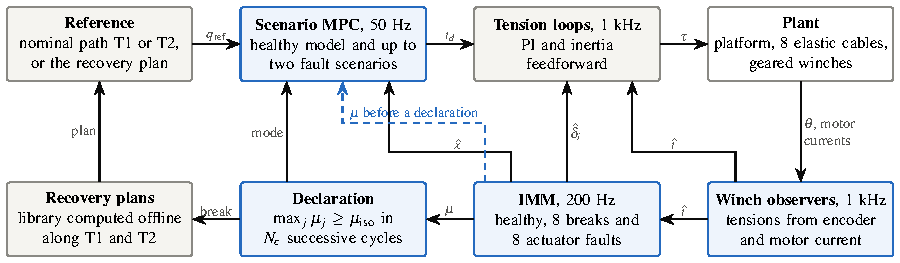
\includegraphics[width=0.86\textwidth]{fig03_architecture.pdf}
\caption{The fault tolerant controller. The winch observers estimate the tensions $\hat{\vc t}$ from the encoder angles and motor currents; the IMM, driven by the tension commands $\vc t_d$ and fed with $\hat{\vc t}$ and the encoder lengths, returns the mode probabilities $\vc\mu$, the platform state $\hat{\vc x}$ and, for an actuator fault, the deficit $\hat\delta_i$ that the tension loop of that winch compensates. Before a declaration the MPC can weight up to two fault scenarios by their probabilities (dashed); after a break declaration its reference becomes the recovery plan stored for that cable and instant.}\label{fig:architecture}
\end{figure*}

\begin{algorithm}[t]
\caption{One cycle of the controller}\label{alg:cycle}
\small
\begin{algorithmic}[1]
\Require read the encoder angles and motor torques of the previous sample
\State update the observer \eqref{eq:eso} of every winch; $\hat t_i\gets-I_mz_{3,i}/r_d-\hat\delta_i$ if winch $i$ is declared faulty
\If{5~ms have passed since the last IMM cycle}
  \State run the IMM \eqref{eq:mix}--\eqref{eq:mu} with the averaged commands; obtain $\vc\mu$, $\hat{\vc x}$, $\hat\delta_i$
  \If{no fault is declared and $\mu_j\ge\mu_{\mathrm{iso}}$ in $N_c$ cycles for one $j\ne0$}
    \State declare $j$; the MPC predicts with mode $j$ from now on
    \If{$j=\mathcal B_i$} \State take the plan of cable $i$ for the instant nearest $t-15$~ms; scale the MPC weights \EndIf
  \EndIf
\EndIf
\If{20~ms have passed since the last MPC solve}
  \State solve \eqref{eq:mpc} from $\hat{\vc x}$ (scenarios from $\vc\mu$ before a declaration); obtain $\vc t_d$, $\ddot{\vc\theta}^{\,\mathrm{ff}}$
\EndIf
\State apply the tension loop \eqref{eq:loop} of every winch
\end{algorithmic}
\end{algorithm}

\subsection{Model predictive control with fault scenarios}\label{sec:mpc}

At each control instant the scenario set $\mathcal J=\{0\}\cup\{j:\mu_j\ge\mu_s\}$ holds the healthy mode and the fault modes whose probability exceeds $\mu_s=10^{-3}$, at most the two most probable ones, with weights $\tilde\mu_j=\mu_j/\sum_{l\in\mathcal J}\mu_l$. The controller solves
\begin{equation}\label{eq:mpc}
\begin{aligned}
\min_{\vc t_0,\dots,\vc t_{N-1}}\ &\sum_{j\in\mathcal J}\tilde\mu_j\Big[\sum_{k=0}^{N-1}\big(\lVert\vc x^{(j)}_k-\vc x^{\mathrm{ref}}_k\rVert^2_{\mt Q_x}+\lVert\vc t_k-\vc t_{k-1}\rVert^2_{\mt Q_t}\big)\\
&\qquad\quad+V_f^{(j)}(\vc x^{(j)}_N)\Big]\\
\text{s.t.}\ &\vc x^{(j)}_{k+1}=\vc f_d\big(\vc x^{(j)}_k,\vc t^{(j)}(\vc t_k)\big),\quad\vc x^{(j)}_0=\hat{\vc x}^{(j)},\\
&t_{\min}\le t_{k,i}\le t_{\max},\qquad j\in\mathcal J,
\end{aligned}
\end{equation}
where $\vc x^{(j)}_k=(\vc q,\vc\nu)$ is the platform state predicted under mode $j$, $\vc f_d$ is \eqref{eq:NE} discretised over the control period and $\vc t^{(j)}(\cdot)$ the map \eqref{eq:modes}. All scenarios share one tension sequence, so the first command suits every mode that is still plausible. For the healthy mode the terminal cost $V_f^{(0)}$ penalises the distance to the reference; for a fault mode it pulls the predicted pose toward the nearest pose that the remaining cables hold with a margin of 10~N, looked up from sets stored offline. As $\mu_j$ grows, this term starts moving the platform toward the region in which it would survive fault $j$ before the fault is confirmed; we call this the probability aware tightening. \citet{raman2023cable} used IMM weights to blend the outputs of mode specific controllers, whereas in \eqref{eq:mpc} the probabilities weight predicted costs inside one optimisation, so the tension bounds hold whichever mode is true. With the healthy mode alone, \eqref{eq:mpc} is a tracking MPC with tension bounds whose first command also solves the tension distribution problem. In the implementation the predictions also carry the bias wrench $\hat{\vc w}_b$ of the IMM, the stage cost of a fault scenario is scaled by 0.1, and two small terms are added, a pull toward the feedforward tensions of the reference and a penalty on predicted free lengths that approach the ends of their drum windows; the complete formulation is in the repository.

The horizon is $N=12$ steps of 20~ms. The programme is written in CasADi \citep{andersson2019casadi} and solved by IPOPT \citep{wachter2006ipopt} with the exact Hessian, warm started from the shifted previous solution. After a break declaration the velocity weights are scaled down and the weight of the tension changes up (Table~\ref{tab:settings}), because the elasticity of the cables, which the prediction model leaves out, matters more with seven cables: at the end poses of the recovery plans the lowest elastic mode of the platform falls to 3.2 to 3.6~Hz, against 5.5~Hz at the home pose with eight cables. We do not claim recursive feasibility or closed loop stability for \eqref{eq:mpc}. The plant differs from the prediction model through the cable elasticity, the winch dynamics and the estimation errors, and the scenario set changes with time. The tension box itself never becomes infeasible, since it does not depend on the state; what can be lost is the ability to track, and the evaluation measures it instead of assuming it.

\subsection{Accommodation of actuator faults}\label{sec:accommodation}

After the declaration of an actuator fault $\mathcal A_i$ the reference is kept, and the tension loop of winch $i$ is corrected by the deficit that the filter of the declared mode estimates, $\hat t_i\leftarrow\hat t_i-\hat\delta_i$ in \eqref{eq:loop}. After a break declaration the winch of the broken cable is held at its angle, so that it does not run away once its load is gone.

\subsection{Recovery after a break}\label{sec:planner}

Once a break of cable $i$ is declared, the planner decides what the platform can still do, in two branches tried in order. In the first, time scaling, the remaining reference over the next 2~s is slowed down by the largest factor $\kappa\in[0.25,1]$ for which the margin \eqref{eq:margin}, with the inertial wrench of the slowed motion added to gravity, stays nonnegative at every sample with the seven cables. Below $\kappa=0.25$ the task no longer continues in any useful sense, and the second branch, recovery, brings the platform to rest within $T=1$~s at a pose the remaining cables hold with a margin of $s_{\min}=10$~N. The recovery path solves an optimal control problem on the rigid model with the remaining cables,
\begin{equation}\label{eq:recovery}
\begin{aligned}
\min\ &\lVert\vc q_N-\hat{\vc q}\rVert^2_{\mt Q_q}+h\sum_k w_v\lVert\vc\nu_k\rVert^2+h\sum_k w_a\Big\lVert\frac{\vc\nu_{k+1}-\vc\nu_k}{h}\Big\rVert^2\\
&+w_r\sum_k\lVert\vc t_{k+1}-\vc t_k\rVert^2+w_s\sum_k s_k\\
\text{s.t.}\ &\vc x_0=\hat{\vc x},\ \ \text{collocation of \eqref{eq:NE} on every interval},\\
&t_{k,i}=0,\quad t_{\min}+s_p-s_k\le t_{k,l}\le t_{\max}-s_p+s_k,\ \ l\ne i,\\
&s_k\ge0,\quad\lVert\dot{\vc p}_k\rVert\le v_{\max},\quad\lVert\vc\varphi_k\rVert_\infty\le25^\circ,\quad\vc\nu_N=\vc0,\\
&\mt W(\vc q_N)\vc t_{\mathrm{hold}}+\vc w_g(\vc q_N)=\vc 0,\quad\lVert\vc\varphi_N\rVert_\infty\le20^\circ,\\
&t_{\min}+s_{\min}\le t_{\mathrm{hold},l}\le t_{\max}-s_{\min},\ \ l\ne i,
\end{aligned}
\end{equation}
transcribed by Hermite--Simpson collocation \citep{kelly2017collocation} on 15 intervals of $h=T/15$ with the tensions constant over each, and solved with IPOPT. The terminal conditions say that the platform ends at rest at a pose the remaining cables hold, and the first term picks among those poses one close to the pose at the break. The twist and acceleration terms keep the motion direct and smooth, and the hard margin $s_p=5$~N is relaxed by slacks $s_k$, so the problem stays feasible from any state; nonzero slacks mark a third branch, a descent with the least violation of the bounds. Three constraints of the implementation are left out of \eqref{eq:recovery} for clarity: a soft tension margin of 20~N, penalised quadratically, which keeps tension in reserve for the feedback of the MPC, the acceleration limit of Table~\ref{tab:parameters}, and the drum windows of the remaining cables. We first joined the current state to the nearest safe pose with a quintic polynomial, but after an upper cable break no duration made such a path feasible, because the seven cables can only produce accelerations inside a narrow set that changes with the pose, and a polynomial of fixed shape does not stay in it.

\subsection{A library of recovery plans}\label{sec:library}

Solving \eqref{eq:recovery} took 0.21~s in the median and at most 0.82~s on one core, and the platform falls during that time. Because the reference paths of a task are known before the task runs, the planner is therefore evaluated in advance. For each path and each cable, the branch and the plan are computed for break instants every 50~ms from 2.5 to 8.0~s, which covers the possible onsets with room for the detection delay. On a declaration at $t_d$ the controller takes the plan of the instant nearest to $t_d-15$~ms, the typical delay of a break declaration, and passes it to the MPC as the new reference together with its tensions as feedforward. Every plan after an upper cable break needed the recovery branch, with a median drop of the reference point of 0.54 to 0.60~m depending on the cable, whereas after a lower cable break the time scaling sufficed for 31 to 69 of the 222 instants of both paths and the recovery plans dropped by at most 0.02~m. The platform hanging from seven cables is unstable along these paths: integrated in open loop with the plan's tensions, it drifts from a recovery path after an upper cable break by up to 0.11~m by its end, so the plan has to be tracked in closed loop. The library assumes a known task; for other states the planner can still be solved online, and the evaluation includes that variant with its latency.

% =====================================================================
\section{Evaluation}\label{sec:evaluation}

\subsection{Simulator}\label{sec:simulator}

The simulator integrates the full model of Section~\ref{sec:model}: the rigid platform with its orientation as a unit quaternion, eight elastic unilateral cables \eqref{eq:tension} and eight winches \eqref{eq:winch} with the torque and speed limits of their drives. At every millisecond it switches on a fault whose onset has been reached, reads the sensors, hands the controller the reading of the previous sample and integrates the plant over the millisecond in 16 Runge--Kutta steps of 62.5~$\mu$s, a step fixed by a convergence test. The plant was verified against a stiff reference solution and against an independent model in MuJoCo \citep{todorov2012mujoco} (Appendix~\ref{app:verification}). The controller never reads the plant state, and it uses the nominal parameters and the rigid model \eqref{eq:NE}; the gap between plant and prediction model is the one any model based controller meets on a real robot, and keeping it prevents the controller from being tested against its own design model. A run counts as a lost platform, and stops, when a tilt angle exceeds $30^\circ$, when $P$ leaves the interior of the frame, or when the drum of an intact cable leaves its window.

Every setting of every method was fixed on calibration runs that share no parameter draw, noise sequence or fault onset with the evaluation, and the protocol of the evaluation, with its methods, runs, endpoints and statistics, was written before any evaluation run. It was amended once: the first evaluation runs showed that the gains of the threshold baseline had been chosen by a rule that ignored the tension bounds, so its settings were chosen again on calibration runs and the evaluation was restarted from its first run, with no setting of any other method changed.

\subsection{Methods compared}\label{sec:methods}

Table~\ref{tab:methods} lists the nine methods that we tested and compared. The ablations A1, A2 and A3 remove one part of the proposed controller P each: the probability aware tightening, the replanning after a break, and the library, whose plan A3 solves online and applies after a latency of 0.4~s, which covers the 99th percentile of the solve times. B0 has no fault tolerance, and the oracle B1 is told the true fault at its onset, which bounds what a perfect diagnosis would achieve with the same controller.

\tablefile{tab_methods}

The threshold baseline B2 stands for the classical pipeline: thresholds on the winch quantities for the diagnosis, a computed torque law with the tension distribution \eqref{eq:margin} instead of the MPC, and the same plan library as P. A baseline is informative only if it is tuned with the same care as the method it is compared with, so its gains and thresholds were chosen on calibration runs of its own controller. It declares a break when the tension estimate of a winch falls below 9~N. Every threshold on the tension residual that detected an actuator fault also raised false alarms with this controller, so B2 does not isolate actuator faults; it is a break detector, which is what the classical literature on cable robots offers.

The learned baseline B3 replaces the mode probabilities of the IMM by those of a recurrent classifier for the declaration, while the filters of the IMM keep running as the state estimator, so that B3 differs from A1 in the diagnosis alone. In B3T the classifier's probabilities also weight the fault scenarios of the MPC, as the IMM's do in P. The classifier has the same seventeen classes as the IMM and sees the same information: at every estimator cycle, the tension residual $\hat t_i-t_{d,i}$, the tension estimate $\hat t_i$ and the deviation of the free length from its value at the reference pose, for each winch. A long short term memory network \citep{hochreiter1997lstm} of two layers of 64 units reads the last 0.1~s of these 24 channels; its architecture and hyperparameters came from a search of 30 trials on validation runs \citep{akiba2019optuna}. It was trained on 528 runs of both paths, recorded with the controller without tightening and with declarations disabled, so that the motion carries no trace of any diagnosis. Its outputs were calibrated by temperature scaling \citep{guo2017calibration}, and the declaration rule of the IMM was applied to them with thresholds chosen on validation runs.

\subsection{Runs, metrics and statistics}\label{sec:protocol}

Every fault type was injected on every cable of both paths in 13 repetitions: a break, a loss of effectiveness of $\rho=0.3$ or 0.6, and a torque bias of $\pm10\%$ of the holding torque, 624 fault runs in all, with the onset drawn uniformly between 3 and 7~s and the run ending 4~s after it or when the platform is lost. There were 100 fault free runs of 16~s per path. Each run draws its plant parameters from its seed (Table~\ref{tab:parameters}), and the current noise is nominal in half of the runs and doubled in the other half. All methods ran on the same seeds, so every comparison is paired. Counting every method on every run it applies to, B3T on a subset fixed in advance, the evaluation comprises 5,212 simulations.

Errors are taken to the active reference, the nominal path before a declaration and the plan after it, and the transient is the 2~s after the onset. The diagnosis is scored by the declared mode, its delay and the false alarms, declarations before the onset or in a fault free run counted per hour of operation with the fault modes armed. The recovery time is the time from the onset after which the position error stays for 1~s within twice the 95th percentile of the error in the fault free runs of the same path. Six primary endpoints were fixed with their comparisons, each with a Holm correction \citep{holm1979}: the platform lost after a break, the fault declared with the correct mode, the delay of the correct declarations, the false alarms per hour, the smallest tension margin in the transient and the share of the transient outside the bounds. Shares carry 95\% Wilson intervals \citep{wilson1927} and paired comparisons McNemar's exact test \citep{mcnemar1947}; continuous endpoints are compared with the Wilcoxon signed rank test \citep{wilcoxon1945} and bootstrap intervals \citep{efron1993bootstrap}. No run was excluded.

% =====================================================================
\section{Results}\label{sec:results}

Table~\ref{tab:results} gives the outcome of every method; the complete statistics of the six endpoints are in the repository given under Data availability.

\tablefile{tab_results}

\subsection{One break in detail}\label{sec:example}

Fig.~\ref{fig:example} follows one break, chosen by a rule fixed before drawing: among the upper cable breaks whose traces were kept, the run with the median declaration delay of P. Cable~2 breaks at 4.933~s on T1. The IMM gives the break mode a probability above 0.99 in the cycle 11~ms after the break and declares it after 17~ms. The classifier's probability rises earlier, to 0.99 at 6~ms, but both reach the threshold of 0.9999 in the same cycle, 11~ms after the break; the IMM needs two such cycles and declares after 17~ms, the classifier needs four and declares after 27~ms, and the threshold rule of B2 declares at 22~ms. The platform cannot stay where it is. Under P it descends by 0.5~m along the recovery plan to a pose the seven remaining cables can hold, tilting by at most $6.7^\circ$ and settling at $5.3^\circ$, while the seven intact cables take over the load of cable~2: an intact cable leaves its bounds for 5\% of the first 2~s, all of it within 0.21~s of the break, and from 0.3~s on every intact tension lies between 15 and 183~N. Without fault tolerance the platform turns past $30^\circ$ and is lost 0.40~s after the break.

\begin{figure*}[t]
\centering
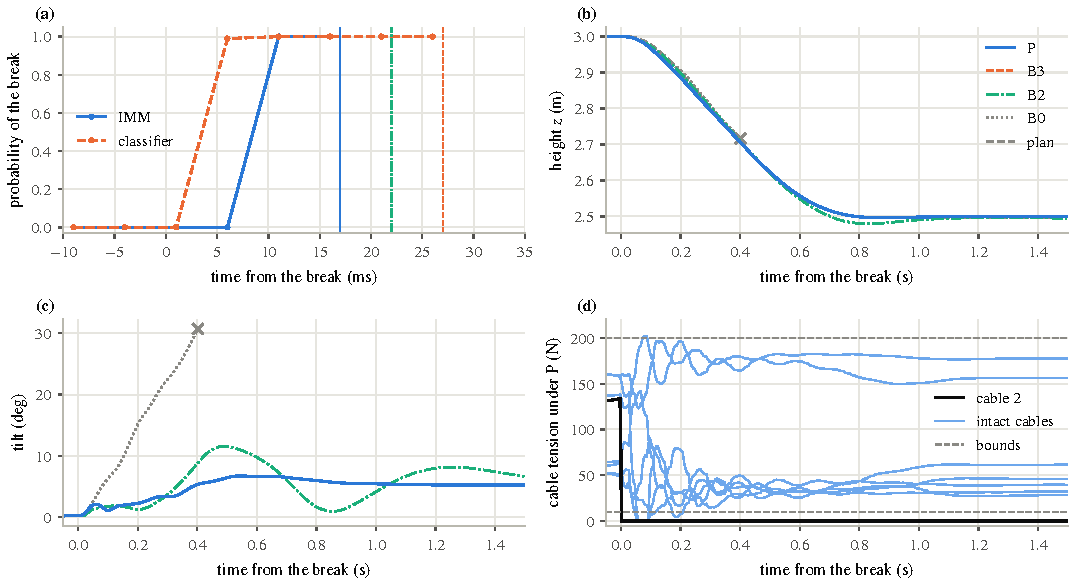
\includegraphics[width=\textwidth]{fig04_example_break.pdf}
\caption{A break of the upper cable~2 at 4.933~s on T1 (run 1 of the evaluation), drawn from the stored traces. (a) Probability of the true mode from the IMM and from the classifier up to their declarations; vertical lines: declarations of P (17~ms), B2 (22~ms) and B3 (27~ms). (b) Height of the platform and the recovery plan followed by P. (c) Tilt; the cross marks the loss of the platform without fault tolerance (B0). (d) Cable tensions under P with the tension bounds: the seven intact cables take over the load of the broken one. The curves of B3 lie under those of P.}\label{fig:example}
\end{figure*}

\subsection{Detection and isolation}\label{sec:detection}

The IMM declared 623 of the 624 faults with the correct mode (Fig.~\ref{fig:delays}). Its median delay was 17~ms for a break, 23~ms for a loss of effectiveness and 41~ms for a bias, and no break took longer than 19~ms. Its one false alarm, 2.8~s before a loss of effectiveness of the same winch, is also the one fault it did not declare correctly. On the same runs P declared 5~ms earlier than B2 and 10~ms earlier than B3 (paired medians). B2 declared every break correctly and no actuator fault, and in 21 runs with a loss of effectiveness of an upper winch it declared a break of a healthy lower cable whose tension had fallen below its threshold. The classifier of B3 declared all 208 breaks correctly, 206 of the 208 losses of effectiveness and 184 of the 208 biases.

\begin{figure*}[t]
\centering
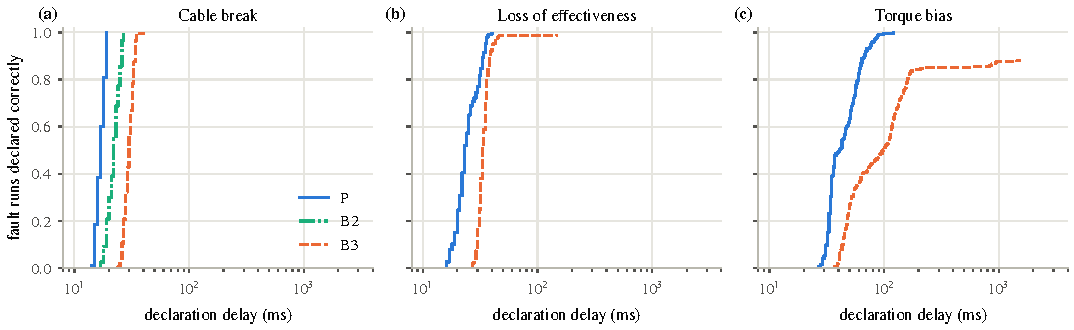
\includegraphics[width=\textwidth]{fig05_detection_delay.pdf}
\caption{Share of the 208 fault runs of each type (both paths) declared with the correct mode within a given delay after the onset. The IMM (P) declares every break within 19~ms and isolates losses of effectiveness and biases faster and more completely than the classifier (B3); the threshold rule (B2) isolates breaks only. A curve ends at the share of correct declarations.}\label{fig:delays}
\end{figure*}

The difference that matters most in closed loop is the false alarm. The classifier raised 42 false alarms in the 1.29~h of operation in which P raised one, and its fault free runs carried a false alarm in 4 of 100 on T1 and in 34 of 100 on T2 (Fig.~\ref{fig:falsealarms}). Training on both paths brought its isolation close to that of the IMM, but not its rate of false alarms on the helix (Fig.~\ref{fig:learned}). A first classifier trained on T1 alone had shown how strongly the learned diagnosis depends on its training data: on the helix it raised a false alarm in 6 of 8 fault free test runs and declared 45 of 80 faults correctly, taking the healthy motion along the climbing path for actuator faults of the lower winches, while the IMM, which uses a model of the robot rather than examples of its motion, kept its performance on both paths.

\begin{figure}[t]
\centering
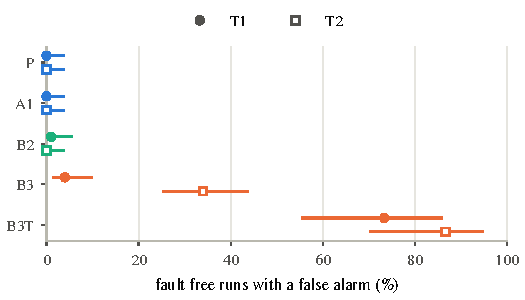
\includegraphics[width=\columnwidth]{fig06_false_alarms.pdf}
\caption{Share of the fault free runs with a false alarm, with 95\% Wilson intervals (100 runs of 16~s per path; 30 per path for B3T). The IMM raised none with or without the tightening; the classifier raised many on the helix T2, and many more when its probabilities also weighted the MPC (B3T).}\label{fig:falsealarms}
\end{figure}

\begin{figure*}[t]
\centering
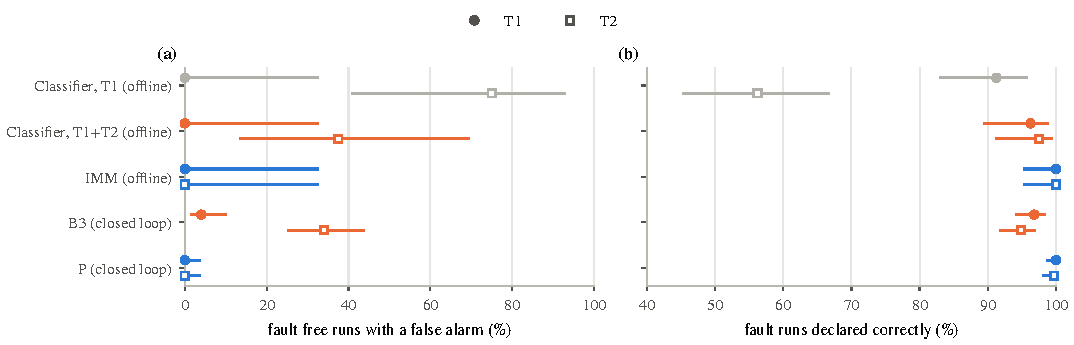
\includegraphics[width=\textwidth]{fig07_learned_vs_model.pdf}
\caption{Learned against model based diagnosis, offline and in closed loop, with 95\% Wilson intervals. (a) Fault free runs with a false alarm. (b) Fault runs declared with the correct mode. Offline: single tests on the same stored runs (8 fault free and 80 fault runs per path) of the classifier trained on T1, of the classifier trained on both paths and of the IMM. Closed loop: the evaluation (100 fault free and 312 fault runs per path). Training on both paths removes most of the failure to generalise to the helix, but the false alarms on T2 remain.}\label{fig:learned}
\end{figure*}

\subsection{Safety after a break}\label{sec:safety}

The proposed controller lost the platform after 11 of the 208 breaks (5.3\%), against 122 without fault tolerance (58.7\%), 65 for B2 (31.2\%), 25 for B3 (12.0\%) and 38 without replanning (18.3\%); every one of these differences remains after the Holm correction. All 11 losses of P followed the break of an upper cable, 6 of 52 on T1 and 5 of 52 on T2, and P kept the platform after every lower cable break (Fig.~\ref{fig:safety}). The oracle B1 lost 4, three of them after upper cable breaks, so even a diagnosis without delay cannot save every upper cable break with this controller. The price of the 17~ms of diagnosis appears in the tension bounds rather than in the losses: during the 2~s after a break a cable was outside its bounds for 5.1\% of the time under P and 2.1\% under the oracle (medians). B2, with its gains tuned on its own calibration runs and the same plans, lost 65 platforms, 30 of them after a lower cable break, after which P never lost one.

\begin{figure*}[t]
\centering
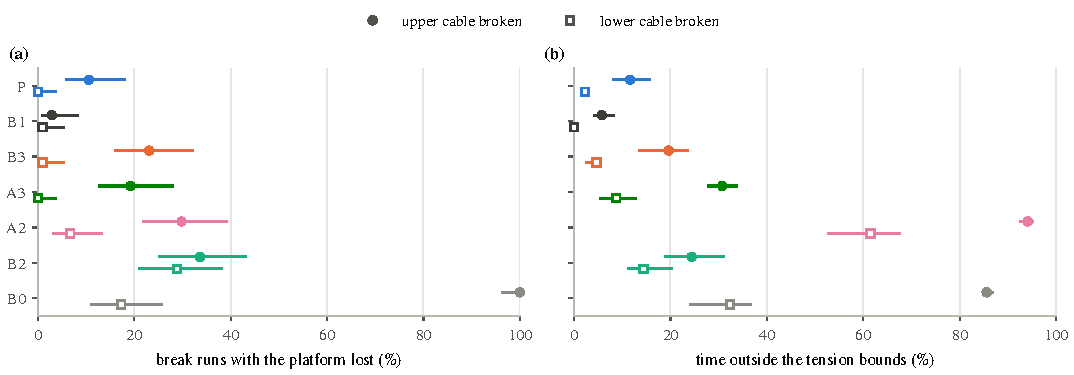
\includegraphics[width=\textwidth]{fig08_safety_after_break.pdf}
\caption{Safety after the 104 upper and 104 lower cable breaks of the evaluation. (a) Share of the runs in which the platform was lost, with 95\% Wilson intervals. (b) Median share of the 2~s after the break during which an intact cable was outside its tension bounds, with 95\% bootstrap intervals. All losses of P follow upper cable breaks; without replanning (A2) the platform spends most of the transient outside the bounds.}\label{fig:safety}
\end{figure*}

\subsection{Recovery}\label{sec:recovery}

Replanning carries most of this result. Without it (A2), 38 platforms were lost, 86.5\% of the transient was spent outside the bounds in the median, and the error after the transient was 72.7~mm against 5.6~mm for P. The library matters as well: solving the plan online with its latency (A3) lost 20 platforms against 11 (paired, $p=0.09$, a secondary comparison) and raised the time outside the bounds in the transient from 5.1 to 20.2\%. With P the position error returned to the band of the fault free runs in 181 of the 208 break runs, after 0.27~s in the median (Fig.~\ref{fig:recovery}); the oracle recovered 197 runs after 0.19~s, A3 173 after 0.70~s and A2 74 after 1.01~s.

\begin{figure}[t]
\centering
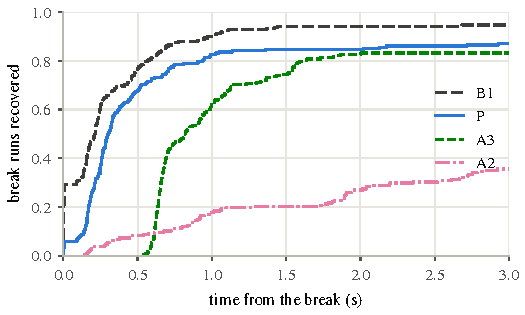
\includegraphics[width=\columnwidth]{fig09_recovery.pdf}
\caption{Share of the 208 break runs whose position error has returned within the given time to twice the 95th percentile of the fault free error of the same path, and stayed there for 1~s. Lost runs and runs that did not recover before their end never reach the curve. The library (P) recovers almost as fast as the oracle (B1); solving the plan online (A3) costs about 0.4~s, and without replanning (A2) most runs do not recover.}\label{fig:recovery}
\end{figure}

\subsection{Actuator faults}\label{sec:actuator}

No method that isolates actuator faults lost a platform after one, except B3T. B2, which cannot isolate them, lost 19 platforms after a loss of effectiveness and 2 after a bias. The accommodation of P is biased, however. After a loss of effectiveness, the IMM's estimate of the deficit had an RMS error of 30~N in the median, 20~N for $\rho=0.3$ and 52~N for $\rho=0.6$, and the error after the transient was 18.2~mm, 14 and 45~mm for the two magnitudes, so that only 80 of the 208 runs returned to the band of the fault free runs. After a bias the deficit error was 5.6~N and 206 of 208 runs returned to the band. The cause is the structure of the accommodation: the IMM keeps the tension commands as its input while the loop of the faulty winch is corrected by the deficit it estimates, so its filter then estimates the deficit that remains after the correction, and the pair settles at about half of the true deficit.

\subsection{The probability aware tightening}\label{sec:tightening}

With the IMM the tightening had no measurable effect (Fig.~\ref{fig:tightening}). P and A1 lost the same number of platforms after a break, 11 each, with the outcome differing in ten runs, five each way; they declared the same faults at the same delays, and their tension margins in the transient did not differ (paired median difference 0~N, $p=0.26$). Before a fault the tightening was almost never active: the position error before the fault was identical in 804 of the 824 paired runs. The reason is the speed of the IMM. Every break was declared within 19~ms, less than the 20~ms period of the MPC, so the MPC solves at most once with intermediate probabilities before it switches to the model of the declared mode. The tightening can only act while the diagnosis is uncertain, and with this diagnosis that interval is shorter than one control period.

\begin{figure}[t]
\centering
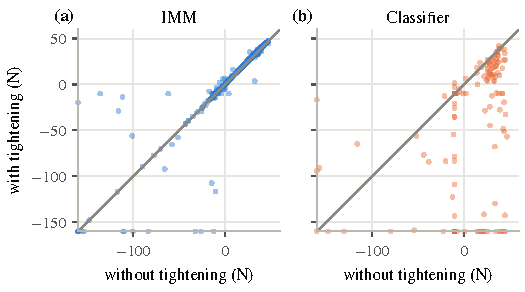
\includegraphics[width=\columnwidth]{fig10_tightening.pdf}
\caption{Smallest tension margin of the intact cables in the 2~s after the fault, with the tightening against without it on the same run. (a) IMM (P against A1, 624 runs): the points lie on the diagonal. (b) Classifier (B3T against B3, 138 runs): most points lie below it. Values below $-160$~N are drawn at $-160$~N.}\label{fig:tightening}
\end{figure}

With the classifier the tightening was harmful. On the runs of B3T, its probabilities in the MPC raised a false alarm in 154 of 252 runs against 11 for B3 on the same runs, reduced the correct declarations from 186 to 16 of 192, lost 44 of 64 platforms after a break against 8, and lowered the margin in the transient by 19~N (paired median; 95\% interval $-28.7$ to $-13.8$~N). The mechanism showed in the first pilot run of B3T: as soon as the classifier gave the fault modes some probability, the MPC tightened toward them, the motion this produced resembled nothing in the classifier's training runs, which were recorded without tightening, and the classifier then declared an actuator fault on a healthy winch.

\subsection{Computation}\label{sec:compute}

The simulation waits for each solve, so the closed loop behaved as if every computation met its period. On the machine of the evaluation, with two runs sharing two cores, they did not all do so (Fig.~\ref{fig:compute}). The estimator cycle of the observers and the IMM took 2.9~ms on average and 5.3~ms at the 99th percentile, against its period of 5~ms. The MPC took 32~ms on average and 65~ms at the 99th percentile, against its period of 20~ms, so the controller as implemented, with CasADi and IPOPT and the models compiled to C, would not run in real time on this machine.

\begin{figure}[t]
\centering
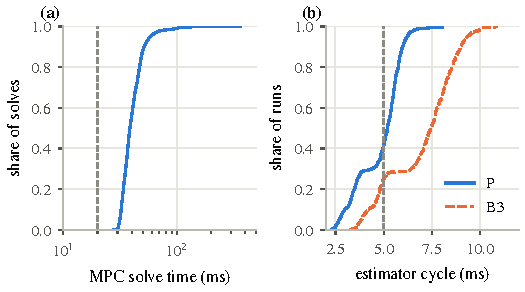
\includegraphics[width=\columnwidth]{fig11_computation.pdf}
\caption{Computation on the machine of the evaluation (two runs sharing two cores). (a) Every MPC solve of P in the kept fault runs against the 20~ms period. (b) 99th percentile of the estimator cycle of every run of P and of B3 (with the classifier) against the 5~ms period.}\label{fig:compute}
\end{figure}

% =====================================================================
\section{Discussion}\label{sec:discussion}

\subsection{Why the model based diagnosis was faster and more reliable}\label{sec:why}

The IMM separates faults through what each mode predicts, and the predictions differ where the physics of Section~\ref{sec:eso} says they should. A break makes the tension estimate of one winch fall to zero while its command does not, which only the break mode of that cable explains, and this is why every break was declared within four estimator cycles. An actuator fault leaves the winch estimate at its command and moves the platform, which the length readings of all eight cables register, so the actuator modes need more evidence and take longer. The filters also take the controller's own tension commands as their input, and so they carry a model of the motion the controller produces. The classifier has no such model. It learned the motion of its training runs, and when the motion differed, on the helix it had not seen or under the tightening, it read the difference as a fault. Training on more varied runs narrows this gap, but in a fault tolerant controller the controller itself creates new motion once it acts on the detector, and that motion cannot be in the training data of a detector trained before the controller used it. Used for the declaration alone, the classifier cost 14 platforms more than the IMM, 25 against 11; used in the constraints of the controller, it lost 44 of 64 breaks. We present B3 as one carefully built learned baseline and not as the best a learned detector can do, since a detector trained on more runs, more paths and runs that include the controller's reaction would do better.

\subsection{What the library buys and what it assumes}\label{sec:librarydiscussion}

The plans of the library are the same plans that the online planner computes; the difference between P and A3 is only when they are available. The 0.4~s of latency cost nine platforms and quadrupled the time outside the bounds, which confirms that after an upper cable break the robot has a fraction of a second, not seconds, to start moving. The price of the library is that it needs the task in advance. For a robot that repeats known paths, as on a production line or a building site where the trajectories are planned before the work, this is a small price, and for other states the online planner remains, with its latency. The remaining losses of P all follow upper cable breaks, and even the oracle lost four platforms. Every plan of the library satisfies the tension bounds, so these losses arise when the closed loop fails to follow a plan that exists, either because the state at the declaration has already drifted from the start of the plan or because the platform on seven elastic cables, with its lowest mode near 3~Hz, does not respond as the rigid model of the MPC predicts. Which of the two dominates we have not analysed run by run.

\subsection{Why the tightening had nothing to act on}\label{sec:tighteningdiscussion}

The tightening of \eqref{eq:mpc} assumes an interval in which the diagnosis suspects a fault without having confirmed it, and with the IMM that interval was shorter than one period of the MPC. It would act with a slower diagnosis, or more precisely with a diagnosis that stays uncertain for several control periods, but the only slower diagnosis we tested, the classifier, made it harmful, because its probabilities were not those of a model of the closed loop. Whether a diagnosis can be slow enough to leave the controller time to hedge and still be calibrated to the motion the hedging produces is a question this study leaves open.

\subsection{Limitations}\label{sec:limits}

The controller does not run in real time. The MPC needed 32~ms on average against its period of 20~ms, because it solves a nonlinear programme with the exact Hessian to convergence at every step. A real time iteration scheme \citep{diehl2005rti}, which performs one sequential quadratic programming iteration per sample, implemented in a solver built for embedded optimal control such as acados \citep{verschueren2022acados}, or a shorter horizon, are the next steps.

The accommodation of actuator faults is biased (Section~\ref{sec:actuator}). Giving the IMM the corrected command removes the bias in the steady state, and in pilot runs it cut the error after a loss of effectiveness of 0.3 from 25 to 2~mm, but it lost the platform for $\rho=0.6$, where the present scheme kept it. An accommodation that estimates the deficit from the corrected command therefore needs a stability argument which the present design does not have.

The study is a simulation. The geometry and inertia of the robot are those of a published model, but the cable stiffness is scaled from a larger cable, the motor is sized from the manufacturer's data, the noise of the current measurement is our choice, and friction is not modelled. Friction in the gearbox and at the drum would enter the tension estimate \eqref{eq:bias} like a torque bias, as an error that changes sign with the winch speed, and would have to be identified and compensated on hardware. The evaluation randomises the parameters and doubles the noise to cover part of this uncertainty, but a test on a physical robot is the step that remains. It also covers single faults only: the IMM and the declaration logic handle one fault and do not rearm after a declaration, so a second fault during the recovery is outside its scope.

% =====================================================================
\section{Conclusions}\label{sec:conclusions}

A cable break on this robot is a race against the fall of the platform, and the race is won by isolating the fault quickly and having the recovery motion ready. A two level diagnosis, observers at the winches and an IMM over seventeen modes at the platform, isolated every fault type from the encoders and motor currents alone, declared every break within 19~ms and raised one false alarm in 1.29~h. With recovery plans computed in advance along the task the platform was lost after 11 of 208 breaks, all of them upper cable breaks, against 122 without fault tolerance and 20 when the same plans were solved online. A learned classifier trained on the same signals was slower and less reliable, and when its probabilities shaped the constraints of the controller the closed loop raised false alarms in most runs. Weighting fault scenarios by the probabilities of the IMM, the idea the study started from, had no effect because the IMM declares a break within one control period. The work stops short of a real time implementation and of an unbiased accommodation of actuator faults, and its next steps are a real time iteration of the MPC, an accommodation with a stability argument, double faults and the test on a laboratory robot that would show whether the margins found in simulation hold on hardware.

% =====================================================================
\section*{CRediT authorship contribution statement}
\textbf{Mfeuter Joseph Tachia:} Conceptualization, Methodology, Software, Validation, Investigation, Writing -- original draft. \textbf{Alexander V. Maloletov:} Supervision.

\section*{Declaration of competing interest}
The authors declare that they have no known competing financial interests or personal relationships that could have appeared to influence the work reported in this paper.

\section*{Funding}
This work was financially supported by the Laboratory of the Institute of Artificial Intelligence, Innopolis University.

\section*{Data availability}
The code of the robot model, the simulator, the estimators, the controller and the learned classifier, the configuration files, the stored results of the evaluation with the complete statistics of its endpoints, and the scripts that rerun every step are available at \url{https://github.com/Tachia/cdpr-fault-tolerant}, the code under the MIT licence and the documents and data under CC BY 4.0.

\section*{Declaration of generative AI use}
During the preparation of this work the authors used Claude (Anthropic), a large language model used through the Claude application with code execution, to write and run the simulation, analysis and plotting code to the authors' design, to draft the manuscript text from the authors' study design and results, and to check the bibliographic records of the references. The figures were rendered by these plotting scripts from the stored simulation results; no figure was generated or altered by the tool itself. After using this tool, the authors reviewed and edited the content as needed and take full responsibility for the content of the published article.

\section*{Acknowledgements}
The authors thank the Laboratory of the Institute of Artificial Intelligence, Innopolis University, for its financial support of this work.

\appendix
% =====================================================================
\section{Verification of the model and the simulator}\label{app:verification}

Table~\ref{tab:verification} lists the checks of the model of Section~\ref{sec:model} and of the simulator. All of them run automatically on the code that produced the results.

\begin{table*}[h]
\centering\small
\caption{Verification of the model and the simulator. The model checks use 100 random poses within $\pm0.5$~m and $\pm0.5$~rad of the home pose; the simulator checks use the parameters of the study.}\label{tab:verification}
\begin{tabular}{@{}p{0.5\textwidth}p{0.18\textwidth}p{0.24\textwidth}@{}}
\toprule
Check & Criterion & Result\\
\midrule
$\partial\vc l/\partial\vc q=-\mt W^\top\mt H$ against central differences & relative error $<10^{-7}$ & $9.0\times10^{-10}$\\
$\mt M=\mt H^\top\mt M_\nu\mt H$ against a symbolic Lagrangian & absolute error & $1.8\times10^{-15}$\\
$\vc G=-\mt H^\top\vc w_g$ against the symbolic gradient & absolute error & $7.1\times10^{-15}$\\
$\dot{\mt M}-2\mt C$ skew symmetric, $\dot{\mt M}$ exact & $<10^{-10}$ & $7.1\times10^{-15}$\\
Lagrange form \eqref{eq:EL} against Newton--Euler form \eqref{eq:NE} & largest difference of $\dot{\vc\nu}$ & $9.9\times10^{-11}$\\
Energy with locked winches and undamped cables, 10~s at 62.5~$\mu$s & drift $<10^{-6}$ of the initial kinetic energy & $3.5\times10^{-11}$\\
Static equilibrium at the home pose & tensions of \eqref{eq:margin} & 151.4 and 58.6~N; largest $|\dot{\vc x}|=4.8\times10^{-10}$\\
Step halving from 62.5 to 31.25~$\mu$s, five fault scenarios & metrics change $<0.1\%$ & all but one ($0.12\%$, the peak tension of an upset platform)\\
Reference solution, Radau IIA \citep{hairer1996stiff,virtanen2020scipy}, lower cable break & & $5.8\times10^{-8}$~m, 0.010~N\\
Independent model in MuJoCo, same inputs, slack cables, 5~s & difference $<1\%$ of the motion & $1.4\times10^{-10}$ of the motion\\
\bottomrule
\end{tabular}
\end{table*}

\FloatBarrier

\bibliographystyle{elsarticle-num-names}
\bibliography{references}

\end{document}
